%# -*- coding: utf-8-unix -*-
%%==================================================
%% chapter01.tex for SJTU Master Thesis
%%==================================================

%\bibliographystyle{sjtu2}%[此处用于每章都生产参考文献]
\chapter{建立SpamTracer检测模型}
\label{chap:model}


\section{模型整体结构}

本章我们要介绍SpamTracer水军检测模型的设计结构和设计理念。如图~\ref{fig:structure}所示为SpamTracer模型的水军检测流程图。整个检测流程分为以下四个步骤:

\begin{figure}[htbp]
	\centering
	\begin{minipage}[htbp]{\textwidth}
		\centering
		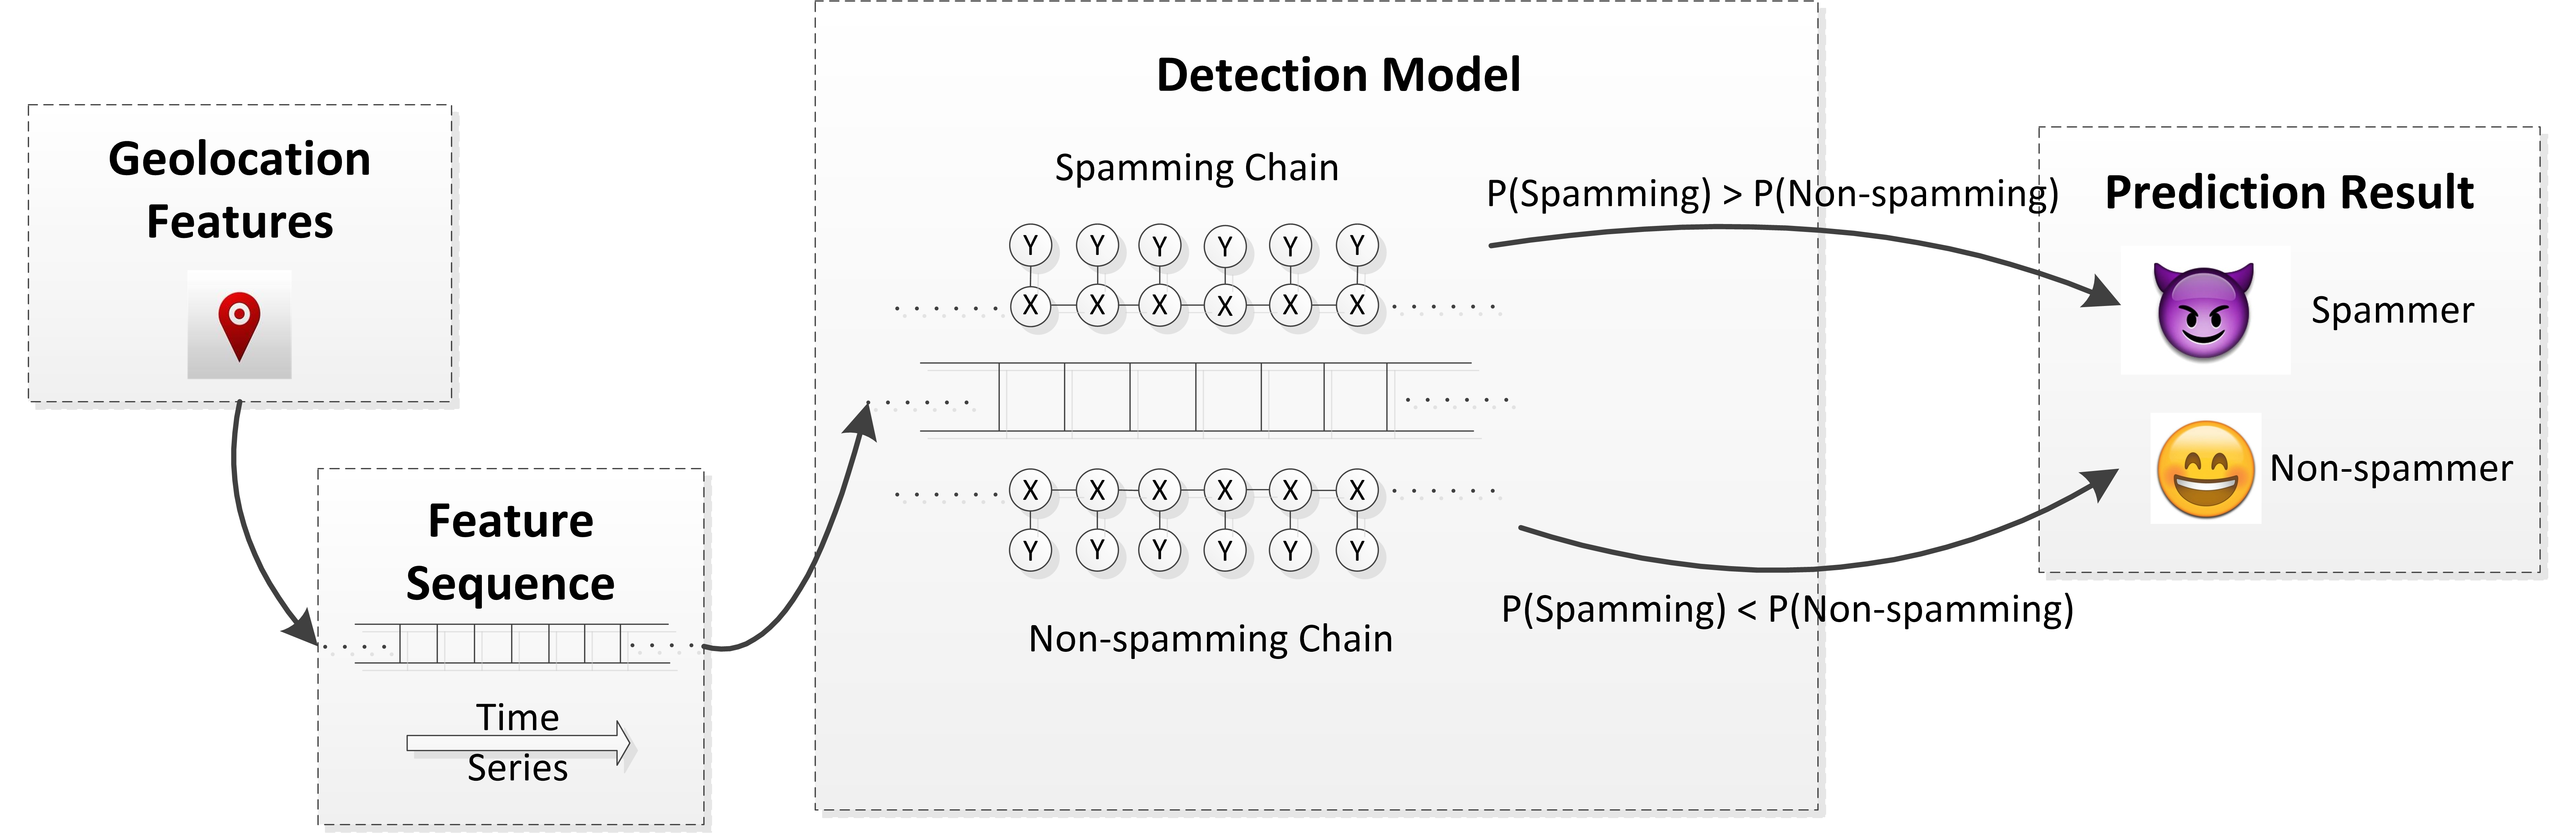
\includegraphics[width=16cm]{model-1.jpg}
		\caption[水军检测流程图]
		{水军检测流程图\label{fig:structure}}		
	\end{minipage}     
\end{figure}

\begin{enumerate}
	\item[(1)] 从数据集中提取地理位置信息数据;
	\item[(2)] 计算每个用户的评论中出现的店铺的地理位置特征,将计算结果按照时间顺序排序,形成特征序列;
	\item[(3)] 将待检测用户的特征序列输入模型;
	\item[(4)] 模型输出该用户是否为水军用户的判断结果。
\end{enumerate}

SpamTracer做出判断的依据是概率。在输入特征序列后,SpamTracer会根据训练出的模型参数,分别计算该序列属于水军用户的概率和普通用户的概率,然后选择概率较大的一方作为判断结果。下文将会叙述地理位置特征的选择,SpamTracer的设计理念,以及模型具体如何对概率进行计算。


\section{选择地理位置特征}

由于发布评论这个事件可以视为是以一个固定的概率稳定并独立发生的,故O2O平台的用户发布评论的过程可以视为一个随机过程。在这个随机过程下,评论相关的特征会遵循一些特殊的分布。例如著名的泊松过程下,时间间隔变量遵循泊松分布。在寻找帮助解决问题的特征时,研究目标特征遵循的分布特点十分有帮助。关于特征的选择,虽然已经有很多特征证明了它们在水军检测中的重要价值,例如时间、活跃量等,但是地理位置特征却被忽略了。地理位置特征是一项在水军检测任务中十分有潜力的特征,如果分别计算普通用户和水军用户的地理位置特征的相关统计数据和分布特点,加以分析并寻找它们之间的不同之处,那么地理位置特征就可以成为解决问题的切入点。经过我们的研究调查,我们发现了一个可用的地理位置特征——“半径”:

\begin{defn}
	\textbf{半径特征}:半径特征指每一个评论中店铺位置点和该用户的活动中心点的距离。其中用户的活动中心点是一个用户的评论列表中最活跃地区内各个店铺位置的地理中心。这个中心点可以被视为该用户的居所。
\end{defn}

图~\ref{fig:radius}是半径特征的示例,图中标有REVIEW LOCATION的点是一个用户写过评论的各个店铺的位置,标有CENTER的点是这些店铺位置的地理中心。我们认为这个点是该用户平时居住的地方,该用户的日常活动是以这个点为中心展开的。图中连接CENTER点和各个REVIEW LOCATION点的线代表了这些点的间隔距离,也就是每个店铺在该用户的评论中对应的半径特征的值。

\begin{figure}[htbp]
	\centering
	\begin{minipage}[htbp]{\textwidth}
		\centering
		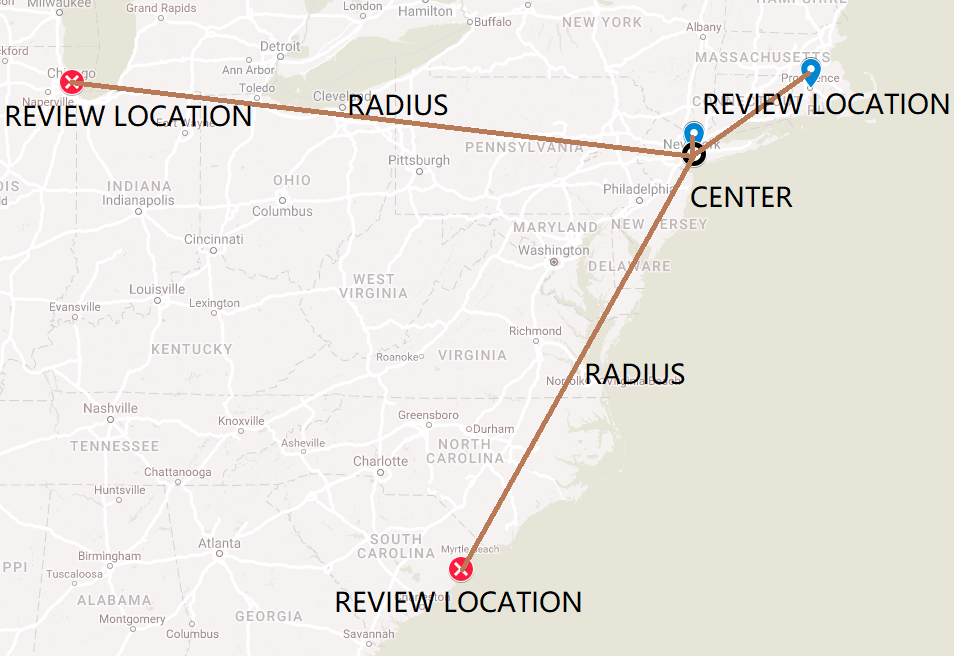
\includegraphics[width=10cm]{featu-1.png}
		\caption[地理位置特征“半径”示意图]
		{地理位置特征“半径”示意图(图源:谷歌地图)\label{fig:radius}}		
	\end{minipage}     
\end{figure}



\section{半径特征的合理性论述}

表~\ref{tbl:radius}和图~\ref{fig:hist}展示了半径特征的统计数据和频率分布直方图。计算数据来源于我们使用的数据集。统计数据中的平均值和标准差表现了半径特征在两类用户之间的差异。频率分布直方图更加具体地展示了水军用户(Spammer)和普通用户(Non-spammer)的差异,包括图像各位置的斜率、各顶点位置等。但是二者的图像也有相似的部分,那就是它们都呈现出了双峰分布的趋势。而这种双峰图像的形成过程可以看做是两个参数不同的高斯分布(Gaussian Distribution)在对数横坐标轴上的叠加。

\begin{table}[htbp]
	\caption{半径特征的统计数据}
	\label{tbl:radius}
	\centering
	\begin{tabular}{ccc}
		\toprule
		& 平均值 & 标准差  \\
		\midrule
		水军用户      & 310.0604  & 678.4959  \\
		普通用户  & 568.5133  &	999.4281 \\
		\bottomrule
	\end{tabular}
\end{table}

\begin{figure}[htbp]
	\centering
	\begin{minipage}[htbp]{\textwidth}
		\centering
		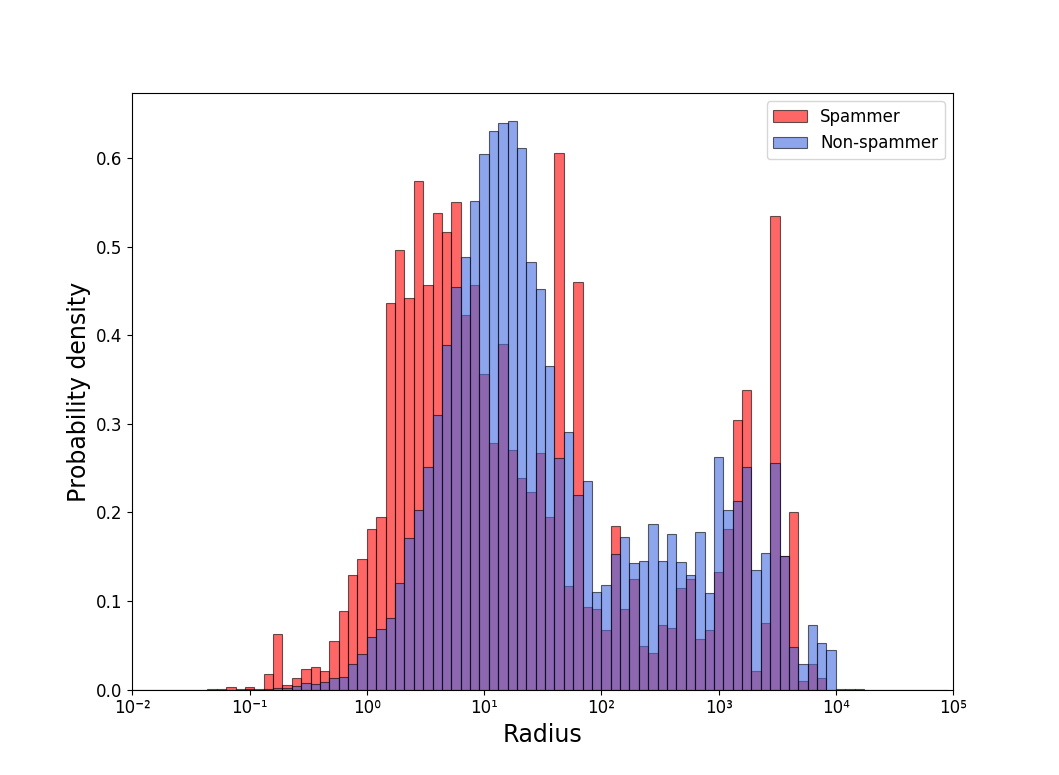
\includegraphics[width=10cm]{featu-2.png}
		\caption[半径特征的频率分布图]
		{半径特征的频率分布图\label{fig:hist}}		
	\end{minipage}     
\end{figure}

从水军用户和普通用户的行为上分析,这种双峰分布是合理的。一般来说,人类的活动范围可以分为两个模式:近距离活动和远距离活动。近距离活动就是人类在居所的附近活动,这类活动占比最高,活动范围不会很远,通常在一个城市的范围之内;远距离活动一般出现在一个人暂时离开居所的时候,例如旅游、出差等,这类活动的地理位置跨越范围较大,但持续时间不会太长。故普通用户图像中的双峰是近距离活动和远距离活动的合理体现。然而,水军用户并不符合近距离活动和远距离活动的模式,他们的行动模式是无规律的,水军用户的双峰图像只是其进行水军活动时不同半径的店铺数量占比的体现。此外,普通用户和水军用户在评论店铺的半径特征顺序上也是有差异的。普通用户评论过的店铺中,连续的店铺的半径特征值基本上是相近的。换句话说,普通用户在店铺的选择上具有空间连续性。这是因为人类的行动是具有空间连续性的,人们在一段时间内是在同一片区域生活的,所以人类日常消费的场所是接近的。即使短时间内出远门旅行,在旅行中的消费场所也是接近的。反观水军用户,其评论店铺的顺序是由雇主要求决定的而非人类正常活动,所以他们的半径特征不具有空间连续性。这两点关键差异将是SpamTracer模型进行水军检测的重要依据。

接下来对半径特征进行数学角度的建模。如上文所提到的,我们用两个参数不同的高斯分布的叠加来描述半径特征的频率分布。假设$x_i, i = 1,...,T$是一个用户的评论列表中按时间排序出现的店铺位置,根据公式~\eqref{equation:1},我们计算其地理中心$C$,然后计算每一个评论的店铺所对应的半径特征值$\gamma_{x_i}$。半径特征值$\gamma_{x_i}$遵循高斯分布。


\begin{equation}
\label{equation:1}
\begin{aligned}
& C = (\frac{\sum_{t \in T}{x_t.latitude}}{|T|}, \frac{\sum_{t \in T}{x_t.longitude}}{|T|})\\
& \gamma_{x_i} = Distance(x_i, C)\\
& f(x;\mu, \sigma) = \frac{1}{\sqrt{2\pi}\sigma}\exp{(-\frac{(x-\mu)^2}{2\sigma^2})} \qquad
\gamma_{x}\sim N(\mu, \sigma^2) \\
\end{aligned}
\end{equation}




\section{建立模型}

接下来我们将叙述如何对地理位置特征进行建模。我们之所以使用半径特征序列而非单独的半径特征,是因为特征序列可以反映上一章所提到的空间连续性,这是分辨普通用户和水军用户的重要依据之一。而且,比起单独的特征,序列形式的特征的有序性可以最大化用户之间的区分度。为了充分利用地理位置特征序列,我们在HMM的基础上进行了改造,设计了处理半径特征序列的监督模型——SpamTracer。

\begin{figure}[htbp]
	\centering
	\begin{minipage}[htbp]{0.6\textwidth}
		\centering
		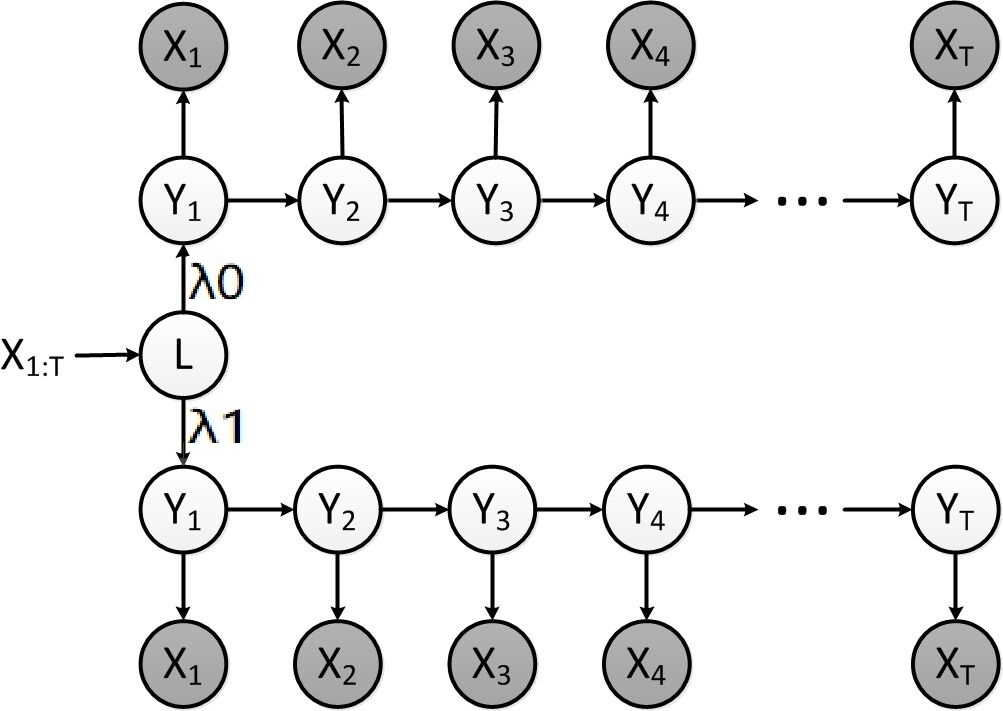
\includegraphics[width=10cm]{model-2.jpg}
		\caption[SpamTracer的双链结构]
		{SpamTracer的双链结构\label{fig:lhmm}}		
	\end{minipage}     
\end{figure}


如图~\ref{fig:lhmm}所示,SpamTracer包含两个HMM子链,以及一个连接两个子链的标签变量。标签变量标记为$L\in\{0,1\}$,其中$0$代表普通用户类,$1$代表水军用户类。两个子链标记为$\lambda_{0}$ = \{$\mathbf{A}_0$, $\mathbf{B}_0$, $\mathbf{\pi_0}$\} 和 $\lambda_{1}$ = \{$\mathbf{A}_1$, $\mathbf{B}_1$, $\mathbf{\pi_1}$\},分别代表普通用户和水军用户,并由相对应类型的数据进行训练。当输入一个新的特征序列时,两个子链会计算各自生成这个序列的概率。这个概率可以视为用来衡量该特征序列与对应子链类别相合程度的分数。分数计算完毕后,模型将比较两个分数的大小,并取拥有较大分数的类别作为判断结果。


\section{模型的合理性分析}


本节我们将从数学角度论证SpamTracer检测过程的合理性。假设有一个位置标签$L$的特征序列$X_{1:T}$输入模型,我们的目的是计算该序列对应标签$L\in\{0,1\}$在不同取值时的产生概率。如公式~\eqref{equation:11}所示,根据贝叶斯公式(Bayes Theorem),计算给定特征序列列$X_{1:T}$条件下标签类型$L = l$的概率$P(L=l|X_{1:T})$可以转化为计算对应子链$\lambda_l$生成给定特征序列列$X_{1:T}$的概率$P(X_{1:T} | \lambda_l)$。此外,公式中的分母部分$P(X_{1:T})$是一个与标签$L$无关的值,故这是一个常量,在比较大小的过程中我们可以忽略它;$P(L = l)$的概率我们可以简单地通过统计数据集中标签为$l$的样本的个数获得。于是问题的关键就在于如何计算不同子链下产生给定特征序列$X_{1:T}$的概率$P(X_{1:T} | \lambda_l)$。

\begin{equation}
\label{equation:11}
\begin{aligned}
\widehat{L} & = \max_{l}{P(L = l| X_{1:T})} \\
& = \max_{l}{\frac{P(X_{1:T} | \lambda_l) \cdot P(L = l)}{P(X_{1:T})}} \quad l\in \{0,1\}
\end{aligned}
\end{equation}

假设$x_i, i = 1,...,T$是一个用户的评论列表中按时间排序出现的店铺位置,$\gamma_{x_i}$代表评论的店铺$X_i$所对应的半径特征值。在SpamTracer的子链中,$\gamma_{x_i}$充当连续的观测态变量$X_i$,即$X_i = \gamma_{x_i}$。$\gamma_{x_i}$遵从两个不同的高斯分布,具体遵从哪一个则是由对应的隐藏态决定的。隐藏态变量值$Y_i$代表$x_i$的模式。$Y_i$有两个可能的取值$\{0,1\}$,分别代表上一章提到的近距离活动模式和远距离活动模式。

子链是由三个参数决定的:初始化概率$\mathbf{\pi}$、转移概率$\mathbf{A}$和输出概率$\mathbf{B}$。初始化概率$\mathbf{\pi} = \{\pi_j\} = \{P(Y_i = j)\}, j \in \{0,1\}$。由于隐藏态的转移概率仅仅依赖于上一个隐藏态,故转移概率如公式~\eqref{equation:3}所示。转移概率可以在模型训练中计算得到。

\begin{equation}
\label{equation:3}
\mathbf{A} = \{a_{jk}\} = 
\begin{bmatrix}
a_{0,0}	&	a_{0,1}	\\
a_{1,0}	&	a_{1,1}	\\
\end{bmatrix}
\end{equation}

观测态变量$X_i$可以直接从数据集中获得,但是$X_i$本质上是由两种不同的高斯分布中的一种生成的,其中高斯分布的种类由对应的隐藏态变量$Y_i \in \{0,1\}$决定。公式~\eqref{equation:5}展示了观测态变量$X_i$是如何服从分布的。

\begin{equation}
\label{equation:5}
X_i = \gamma_{x_i} \sim 
\begin{cases}
N(\mu_0, \sigma_0^2)     &     Y_i = 0	\\
N(\mu_1, \sigma_1^2)     &     Y_i = 1	\\
\end{cases} 	
\end{equation}

与公式~\eqref{equation:1}结合起来看,输出概率$\mathbf{B}$可以用公式~\eqref{equation:6}计算而得。


\begin{equation}
\label{equation:6}
\begin{aligned}	
&b_j(\Delta{x_i})\\
= &P(\Delta{x_i} | Y_i = j)\\
= &f(\Delta{x_i};\mu_j, \sigma_j) \\
= &\frac{1}{\sqrt{2\pi}\sigma_j}\exp{(-\frac{(\Delta{x_i}-\mu_j)^2}{2\sigma_j^2})} \quad j \in \{0,1,2\}\\
\end{aligned}
\end{equation}

综上,我们论述了每个子链$\lambda$及其各自参数$\{\mathbf{A}, \mathbf{B}, \mathbf{\pi}\}$的计算过程,以及如何适配半径特征$\gamma_{x_i}$的分布情况。接下来我们开始计算生成特征序列的生成概率。如果用$X_{1:T}$代表从$x_1$到$x_T$的观测态序列,$Y_{1:T}$代表从$x_1$到$x_T$的隐藏态序列,则公式~\eqref{equation:7}可以计算$X_{1:T}$和$Y_{1:T}$的联合概率。概率$P(X_{1:T}, Y_{1:T})$的含义是$X_{1:T}$和$Y_{1:T}$都按照顺序出现在第$1$到第$T$个位置上的概率。这个计算过程的时间复杂度是$O(T)$。


\begin{equation}
\label{equation:7}
\begin{aligned}
& P(X_{1:T}, Y_{1:T})\\
= & P(Y_1, X_1, Y_2, X_2,...,Y_T, X_T)\\
= & P(Y_1)\prod_{i=1}^{T}{P(X_i|Y_i)}\prod_{i=2}^{T}{P(Y_i|Y_{i-1})}\\
= & \pi_{Y_1}\prod_{i=1}^{T}{b_i(X_i)}\prod_{i=2}^{T}{a_{Y_i Y_{i-1}}}
\end{aligned}
\end{equation}


然而,在实际情况下,对于任意一个给定的观测态序列$X_{1:T}$,我们是不知道它对应的隐藏态序列$Y_{1:T}$的。所以SpamTracer在计算中必须考虑隐藏态序列列$Y_{1:T}$所有的排列组合,共$2^T$中不同的可能性。在这种情况下,计算联合概率的公式如公式~\eqref{equation:8}所示:

\begin{equation}
\label{equation:8}
\begin{aligned}
& P(X_{1:T})\\
= & \sum_{Y_{1:T}} P(X_{1:T}, Y_{1:T})\\
= & \sum_{Y_{1:T}} P(Y_1)\prod_{i=1}^{T}{P(X_i|Y_i)}\prod_{i=2}^{T}{P(Y_i|Y_{i-1})}
\end{aligned}
\end{equation}

如果直接按照上述公式进行计算,时间复杂度将会达到$O(T\cdot2^T)$。这是几乎接近不可计算等级的复杂度。造成如此高计算复杂度的原因主要是该公式对许多中间量进行了冗余的计算。如果能够在计算过程中保存部分中间量,计算将被大大简化。基于这个思路,存在一个经典的Forward-backward算法 \cite{Rabiner:1989}。这个算法可以将公式~\eqref{equation:8}的时间复杂度优化为线性复杂度,大大节省了计算成本。

综上所述,计算不同子链下产生给定特征序列$X_{1:T}$的概率$P(X_{1:T} | \lambda_l)$是完全可行的。我们在理论上证明了SpamTracer是完全可以作为一个监督模型胜任分类工作的。SpamTracer给出的打分可以作为水军检测的依据。


